\section{Instruction Set Architecture}

An \ac{isa} defines the shared behaviour of different implementations of said \ac{isa}. It is an abstract model that guarantees compatibility of software between computers of different implementation. This is called binary intercompatibility. It describes the supported set of instructions, their behaviour, as well as a memory model. The memory model describes the number and roles of all registers, as well as the behaviour of accessing memory and external interfaces. The latter part is also called the ``IO-Model'' of the \ac{isa}. An \ac{isa} may be designed to be extensible or closed for future modifications. 

\subsection{Memory Model}

There are three major, proven memory models for organizing the program and main memory of a computing system:

\begin{itemize}
    \item Von Neumann
    \item Harvard
    \item Modified Harvard
\end{itemize}

In a machine obeying the Von Neumann memory model, there is only one global memory space, which contains both data and program instructions. In a harvard architecture, these memories have a separate address space. A modified harvard architecture is functionally the same as a regular harvard one, but the software can access the instruction memory as if it was data. This is the memory model used by many modern \ac{isa}. For this project, the Harvard memory model is chosen due to its simplicity. The software can be oblivious of the layout of the program memory, which can be directly addressed by a program counter register. This also enables the cell size of the data and program memory to be different, which simplifies instruction addressing and decoding.

The word size of an \ac{isa} is the size of the smallest, atomic unit of data. Since arithmetic operations must be performed on all bits of a word, the number of logic gates and traces scales approximately linearly with the word size. Early processors such as the Intel 4004 had a word size of 4 bits, meaning one word can represent 16 distinct values. However, even in modern systems, the smallest individually addressable unit of bits is the venerable byte, consisting of 8 bits each. It can represent 256 distinct values. Even in modern architectures, the word size is usually an integer multiple of 8. Data larger than the native word size can be emulated by multiple native word length data, which also works for many arithmetic operations.

\subsection{Execution Model}

An execution model describes how the computer achieves computation. This means the order of execution and the number and location of operands and results. As with the memory model, there are multiple options to choose from:

\begin{figure}[htbp]
    \centering
    \begin{subfigure}[b]{0.3\textwidth}
        \centering
        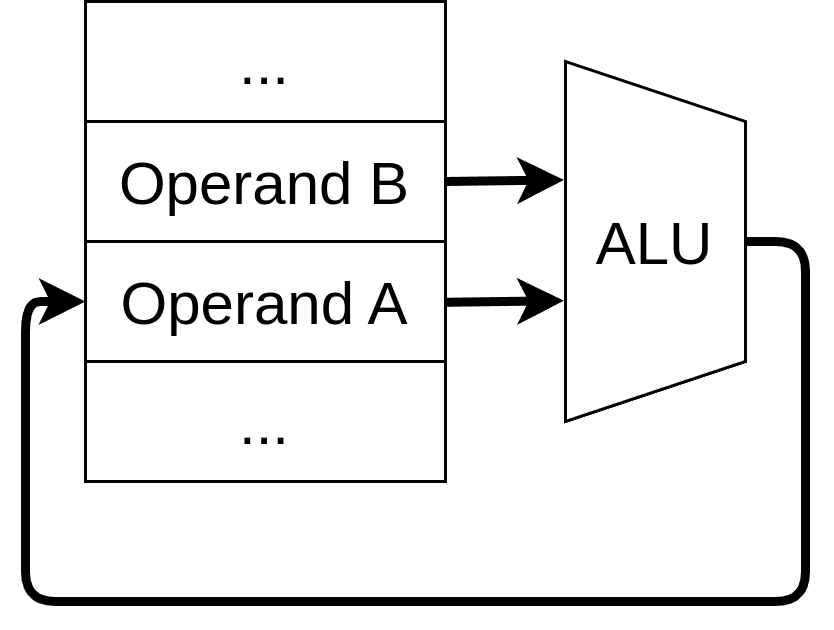
\includegraphics[width=\textwidth]{images/drawio/stack_architecture.png} % Replace with your image file
        \caption{Stack based architecture}
        \label{fig:stack_based_architecture}
    \end{subfigure}
    \hfill % Adds spacing between subfigures
    \begin{subfigure}[b]{0.3\textwidth}
        \centering
        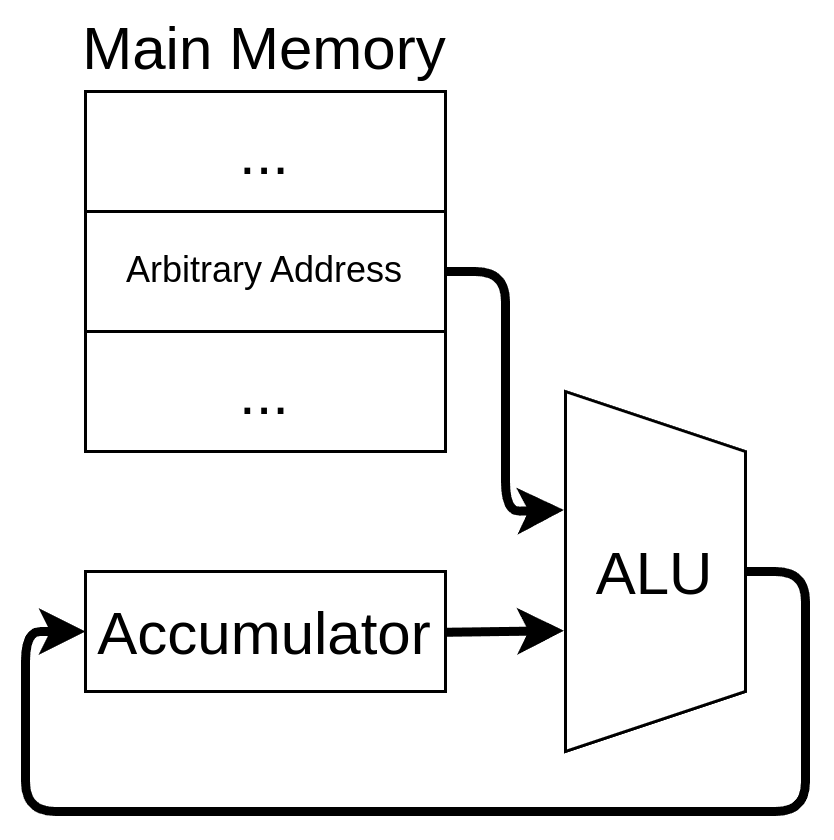
\includegraphics[width=\textwidth]{images/drawio/accumulator_architecture.png} % Replace with your image file
        \caption{Accumulator architecture}
        \label{fig:accumulator_architecture}
    \end{subfigure}
    \hfill
    \begin{subfigure}[b]{0.3\textwidth}
        \centering
        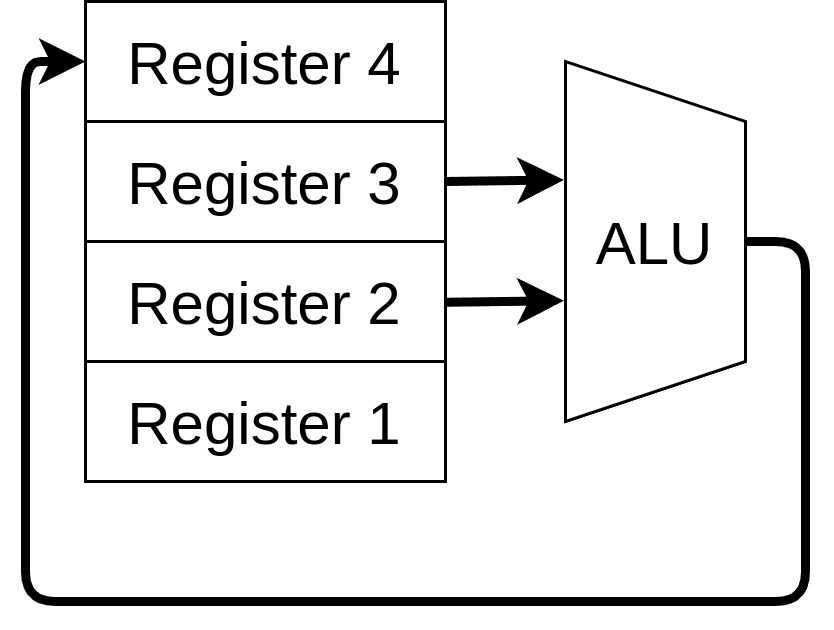
\includegraphics[width=\textwidth]{images/drawio/register_architecture.png} % Replace with your image file
        \caption{Register architecture}
        \label{fig:register_architecture}
    \end{subfigure}

    \caption{Working principle of the three execution models Stack, Accumulator and Register}
    \label{fig:execution_models}
\end{figure}

As shown in \autoref{fig:execution_models}, the stack based model uses a single memory, which is organised by the \ac{lifo} principle. The operands of an operation are always the elements at a specified offset from the stack top. For example, an addition may pop the top two elements off the top of the stack and push the result back ontop. This method has the advantage of not having to specify operand locations in the instruction, allowing for more compact code. However, it lacks the ability to randomly access memory and frequent stack operations can be slow. 

The accumulator-based execution model has a fixed number of registers, one of which is the designated accumulator register. All operations that output a value will store this result in the accumulator register. The accumulator register is also always one of the operands to an operation. The other operand, if required, is read either from memory or from another register, which can either also be fixed or freely chosen by the programmer, depending on the instruction encoding scheme. This execution model is easy to implement and the instructions are also smaller compared to fully addressable operand/destination registers. It is often used in early \ac{cpu} such as the Intel 8008 and 6502 \cite{schlyter200513}. However, its performance is limited by the bottleneck of the accumulator register. it also requires frequent transfers between memory and registers or between registers to save intermediary results, which would otherwise be overwritten by another operation.

The register based execution model provides a fixed set of registers. This model is subdivided further into the ``Register-Register'' and ``Memory-Register'' models. \autoref{fig:register_architecture} shows the former, which is also known as a ``Load-Store architecture'', since the only way of transferring data between registers and memory is via the dedicated load and store operations. All operands and result destinations of an arithmetic operation are registers. The ``Memory-Register'' model allows operations to be read from memory instead. Due to the bottleneck in speed of modern memories, many modern register based architectures are of the Load-Store variant. The register based execution model is highly flexible and well understood. Operands and intermediary results can be reused efficiently and compilers can deterministically optimize register allocation, allowing for higher performance.

\subsection{Addressing modes}

There are many different modes of addressing memories. An addressing mode specifies which memory is accessed, and how the address for that memory is calculated.

\begin{figure}[h!]
    \centering
    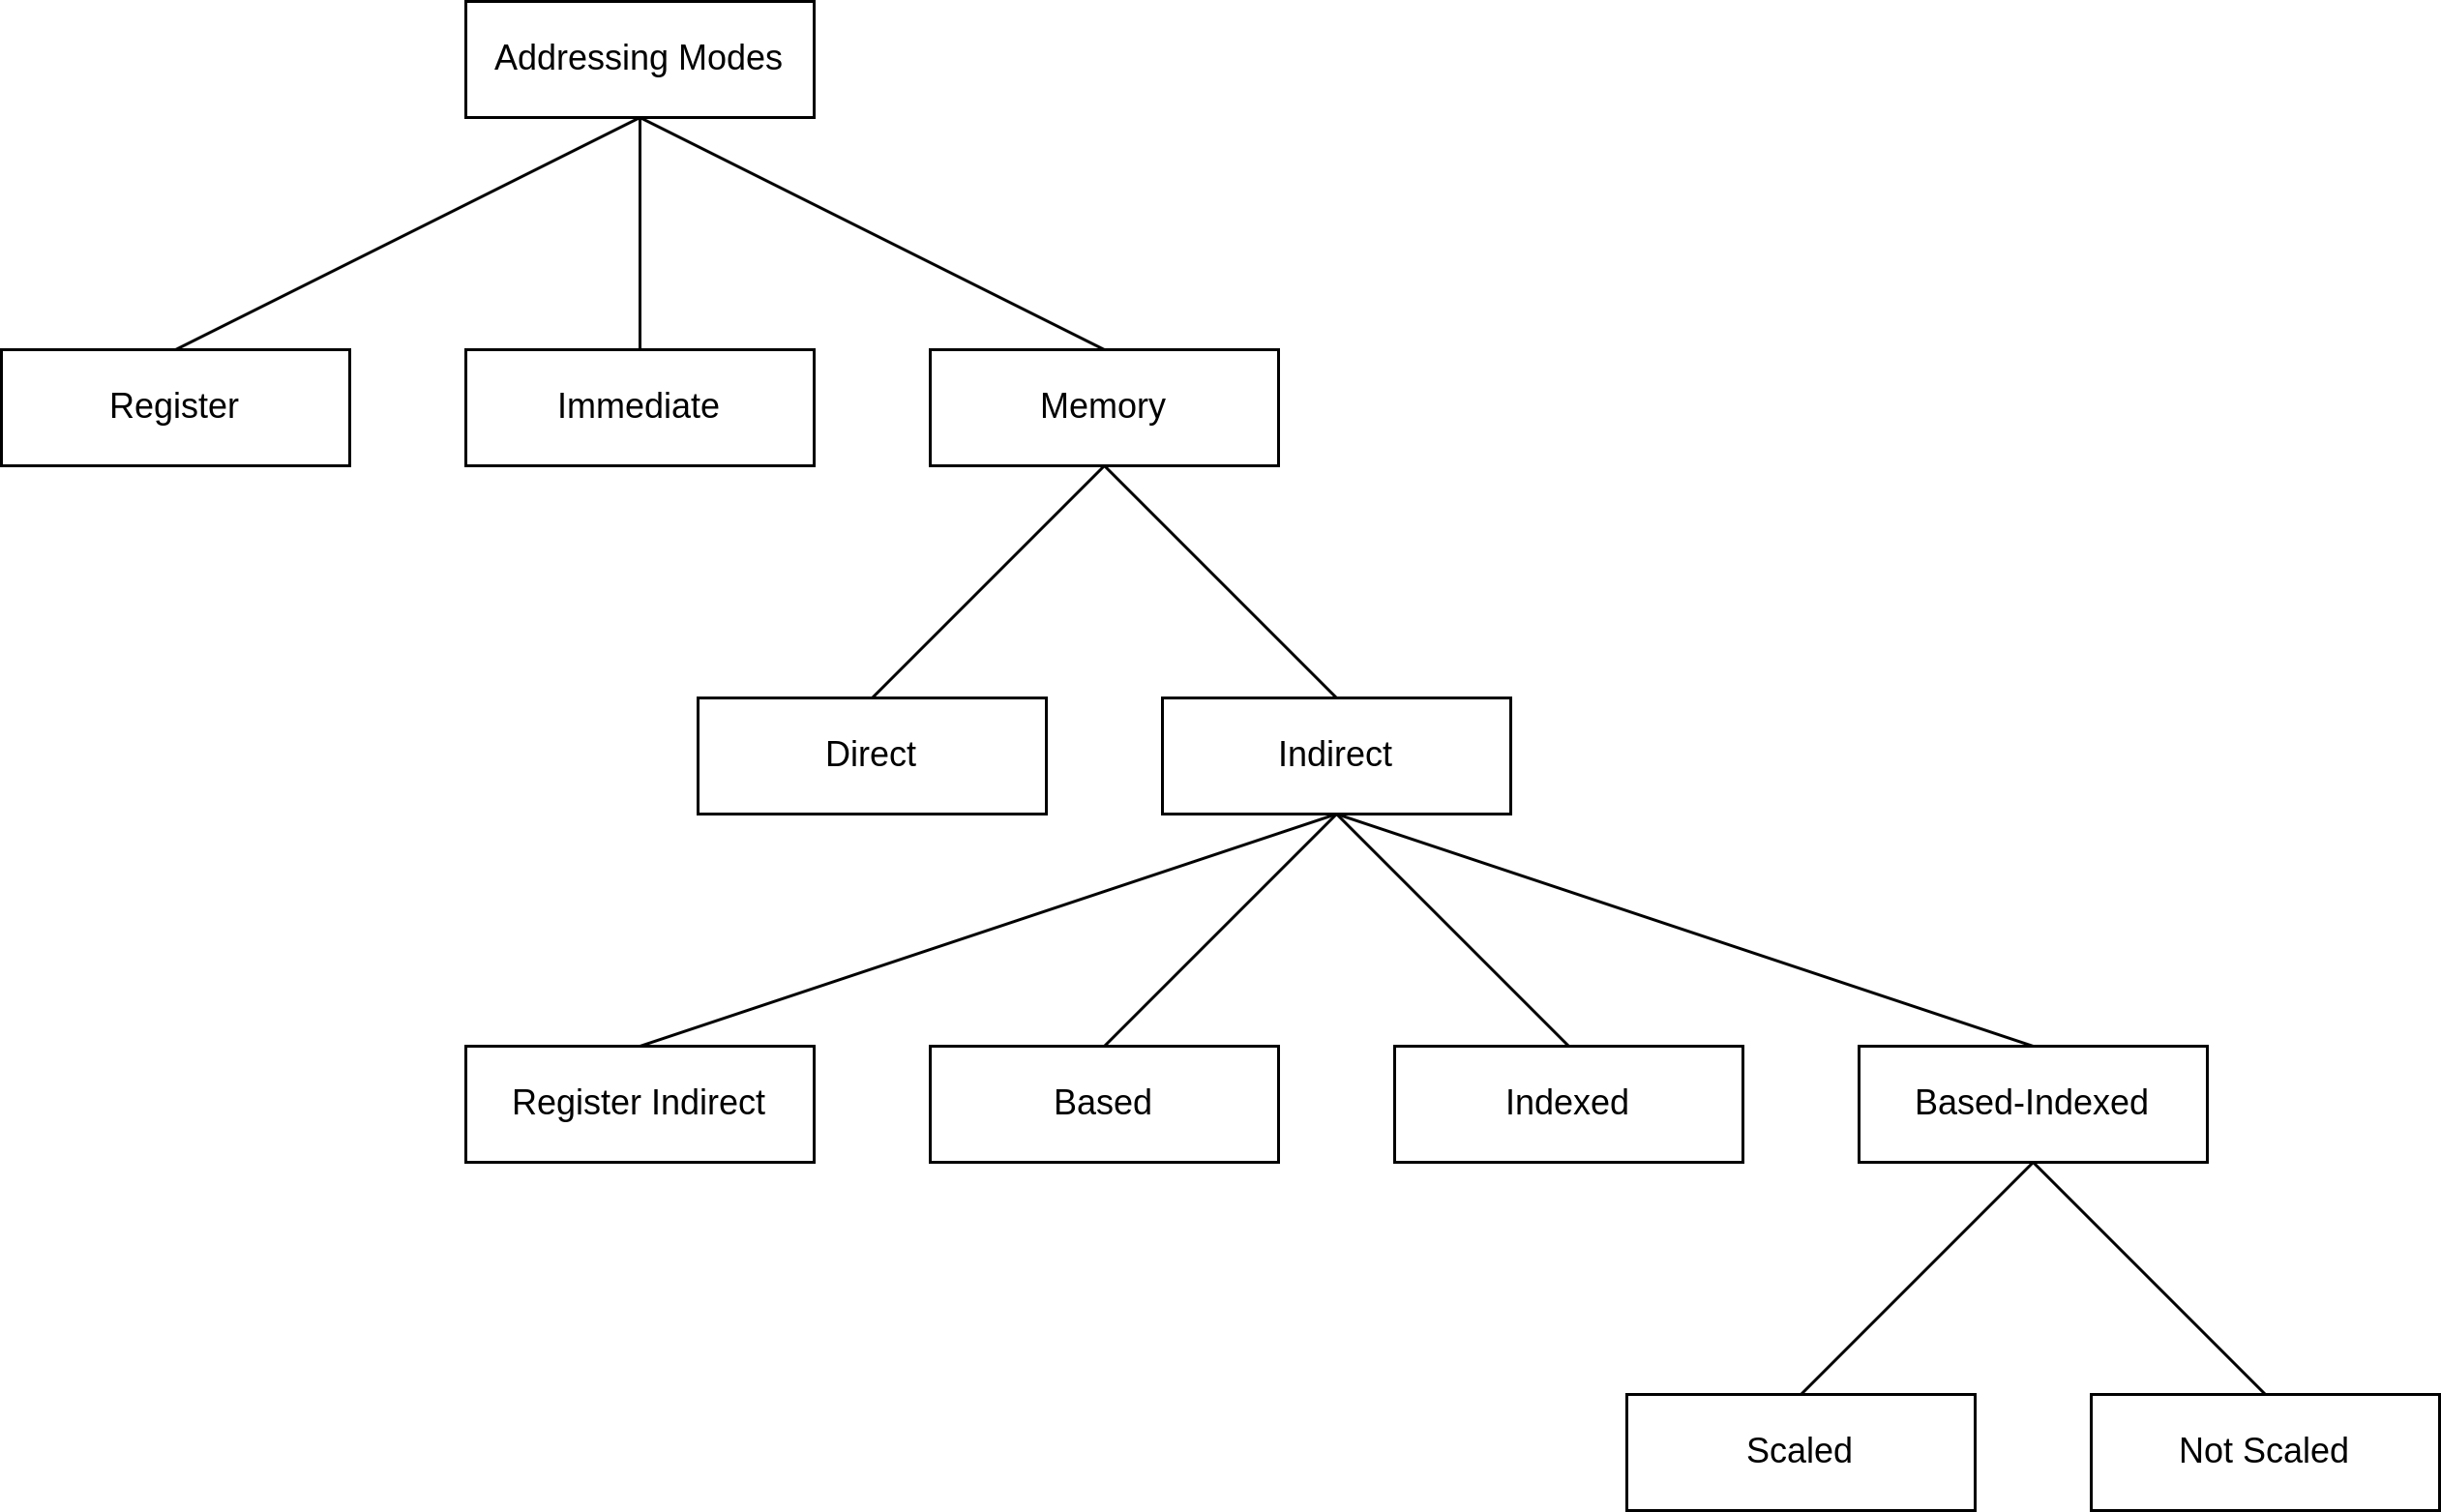
\includegraphics[width=\textwidth]{images/drawio/addressing_modes.png}  % Replace with your image file
    \caption{Hierarchical overview of addressing modes (Modified from S. Dandamudi, omitted more complex addressing modes for brevity \cite{sivarama_addrmodes})}
    \label{fig:addressing_modes}
\end{figure}

\autoref{fig:addressing_modes} shows a hierarchical overview of types of modes of addressing. The complexity and number of arithmetic operations required for each mode increase with each layer. Each layer increases in complexity starting from the left. For example, the most complex mode is referred to as ``Base + Index + Scale + Displacement''. In this mode, the resulting memory address is calculated like so:

$$ \text{Base} + \text{Index} * \text{Scale} + \text{Displacement} $$

This requires additional hardware for performing the additions and multiplication. Note that the ``Scale'' is restricted to 1, 2, 4 or 8 and can therefore be implemented by shifting the index to the left by 1, 2, 3 or 4 bits. In most modern, and some older architectures, the addressing modes can be quite numerous and complex. For example, the Intel 6502 alone has 13 different addressing modes \cite[13.2.1]{schlyter200513}. However, an \ac{isa} need not implement a large number of addressing modes in order to be useful. For example, the Intel 8008 \ac{cpu} only has 3 addressing modes (Register, Register Indirect and Immediate) \cite{cpu-world8008}.

\subsection{Instruction Set}

The instruction set specifies what the \ac{cpu} can do. It contains all available operations and details all operands, affected flags/registers and the effects of the operation when executed. The effects of an instruction can range in complexity.

\subsubsection{Opcodes}

Every instruction is identified by its unique ``Opcode'', which is a discrete number. Based on this number, the processor must infer the number and layout of operands and set up the internal state for execution of the given instruction. The number of bits available for encoding the opcodes determines the maximum number of instructions supported by an \ac{isa}. Not all opcodes within this available range must be assigned. Depending on the design philosophy, unassigned opcodes may be equivalent to NOPs or cause undefined behavior.

\subsubsection{RISC vs. CISC}

Early microprocessors had - by necessity - simple instructions. There were typically also fewer instructions compared to modern systems. This was dictated by the technology at the time. More functionality requires more transistors, which require space on the die, as well as more capabilities for shedding heat. With the shrinking sizes of transistors, more complex instructions became feasible. As with the instructions, the complexity of other systems of a \ac{cpu} grew as well. For example, the Intel 8008 processor released in 1972 \cite{intel4004history} had only 48 instructions \cite{cpu-world8008}, whereas a modern x86 implementation supporting all extensions has $\approx 1795$ instructions \cite[Chapter 7]{heule2016stratified}. Depending on the complexity and number of instructions, an architecture is classified as either \ac{risc} or \ac{cisc}. There is no exact definition of either of these types.

\subsubsection{Types of Instruction}

Instructions can be divided up into different types based on their effects. There are instructions that perform some calculation and store the result in a target memory location. These instructions will be referred to as ``arithemtic instructions''. There are also instructions that do not calculate anything but simply move data between memories. Most \ac{risc} architectures follow the ``Load-Store'' paradigm. This paradigm says that only a select few instructions interact with main memory, whereas the rest of the instructions, including all arithmetic ones, interact only with immediate data and registers. These instructions will be referred to as ``transfer instructions''. Another important class of instruction is the ``control flow instruction''. As the name suggests, this type of instruction usually does not compute anything either, but is responsible for the decision making process within the \ac{cpu}. Upon executing such an instruction, the program counter, instead of being incremented, is overwritten with a value from a memory. This is called branching. There are unconditional and conditional branches, which only overwrite the program counter if some predicate is met. This predicate is typically dictated by a flag stemming from the result of the last arithmetic instruction. Branching is required for implementing function calls and general conditional execution, i.e ``Do X if Y, otherwise do Z''.

\subsection{Instruction Encoding}

A digital processor requires a predefined encoding, according to which the program instructions are formatted. This encoding must include all information required for performing the desired operation. The encoding must include the opcode, all operands and any additional settings required for executing an operation. Since different operations require a different number and type of operand, it can be useful to define a variable length encoding scheme to save memory and increase code density. On the other hand, variable length encodings require additional logic to determine the length from a given opcode and fetch the required number of bytes from memory. This introduces complexity in an implementation, as well as increasing the number of logic gates required. Typically, this also causes the fetch phase to take more than a single clock cycle. For these reasons, many \ac{risc} architectures use a fixed length encoding. Since different types of instructions require different combinations of options and operands, \acp{isa} may define multiple distinct encoding schemes. The instruction decoder can then choose the corresponding format for each opcode, which is usually of a fixed length. 

